% % % % % % % % % % % % % % % % % % % % % % % % % % % % % % % % % % % % % % % %
% IEEE Style - Double columns, 11pt font, letterpaper
\documentclass[journal, twocolumn, final,11pt,letterpaper]{IEEEtran}	

% Include Latex Packages
\usepackage{etex}	% This package enables the use of many packages

% % Page styles
\usepackage{setspace}	% line spacing package
\doublespacing			% use double spacing
%\linespread{1.6}		% Use linespread to fine tune line spacing, not recommended


% % Figures
\usepackage{float}		% improves interface for floating objects
\usepackage{subfig}		% enables subfloat
\usepackage{graphicx}	% more image type support
\usepackage{circuitikz}
\usepackage{epstopdf}	% automatically convert included eps files to pdf
\usepackage{tikz}
%\usepackage{listings}
\usepackage{color}
\definecolor{dkgreen}{rgb}{0,0.6,0}
\definecolor{gray}{rgb}{0.5,0.5,0.5}
\definecolor{mauve}{rgb}{0.58,0,0.82}

\lstset{frame=tb,
	language=Verilog,
	aboveskip=3mm,
	belowskip=3mm,
	showstringspaces=false,
	columns=flexible,
	basicstyle={\small\ttfamily},
	numbers=none,
	numberstyle=\tiny\color{gray},
	keywordstyle=\color{blue},
	commentstyle=\color{dkgreen},
	stringstyle=\color{mauve},
	breaklines=true,
	breakatwhitespace=true,
	tabsize=3
}
\usetikzlibrary{matrix,calc}
\usetikzlibrary{shapes}

\newcommand*{\circled}[2][red]{
	\tikz[baseline=(char.base)]{
		\node[shape=ellipse,inner sep=1pt,
		draw=#1,
		] (char) {#2};}
}

%isolated term
%#1 - Optional. Space between node and grouping line. Default=0
%#2 - node
%#3 - filling color
\newcommand{\implicantsol}[3][0]{
	\draw[rounded corners=3pt, fill=#3, opacity=0.3] ($(#2.north west)+(135:#1)$) rectangle ($(#2.south east)+(-45:#1)$);
}


%internal group
%#1 - Optional. Space between node and grouping line. Default=0
%#2 - top left node
%#3 - bottom right node
%#4 - filling color
\newcommand{\implicant}[4][0]{
	\draw[rounded corners=3pt, fill=#4, opacity=0.3] ($(#2.north west)+(135:#1)$) rectangle ($(#3.south east)+(-45:#1)$);
}

%group lateral borders
%#1 - Optional. Space between node and grouping line. Default=0
%#2 - top left node
%#3 - bottom right node
%#4 - filling color
\newcommand{\implicantcostats}[4][0]{
	\draw[rounded corners=3pt, fill=#4, opacity=0.3] ($(rf.east |- #2.north)+(90:#1)$)-| ($(#2.east)+(0:#1)$) |- ($(rf.east |- #3.south)+(-90:#1)$);
	\draw[rounded corners=3pt, fill=#4, opacity=0.3] ($(cf.west |- #2.north)+(90:#1)$) -| ($(#3.west)+(180:#1)$) |- ($(cf.west |- #3.south)+(-90:#1)$);
}

%group top-bottom borders
%#1 - Optional. Space between node and grouping line. Default=0
%#2 - top left node
%#3 - bottom right node
%#4 - filling color
\newcommand{\implicantdaltbaix}[4][0]{
	\draw[rounded corners=3pt, fill=#4, opacity=0.3] ($(cf.south -| #2.west)+(180:#1)$) |- ($(#2.south)+(-90:#1)$) -| ($(cf.south -| #3.east)+(0:#1)$);
	\draw[rounded corners=3pt, fill=#4, opacity=0.3] ($(rf.north -| #2.west)+(180:#1)$) |- ($(#3.north)+(90:#1)$) -| ($(rf.north -| #3.east)+(0:#1)$);
}

%group corners
%#1 - Optional. Space between node and grouping line. Default=0
%#2 - filling color
\newcommand{\implicantcantons}[2][0]{
	\draw[rounded corners=3pt, opacity=.3] ($(rf.east |- 0.south)+(-90:#1)$) -| ($(0.east |- cf.south)+(0:#1)$);
	\draw[rounded corners=3pt, opacity=.3] ($(rf.east |- 8.north)+(90:#1)$) -| ($(8.east |- rf.north)+(0:#1)$);
	\draw[rounded corners=3pt, opacity=.3] ($(cf.west |- 2.south)+(-90:#1)$) -| ($(2.west |- cf.south)+(180:#1)$);
	\draw[rounded corners=3pt, opacity=.3] ($(cf.west |- 10.north)+(90:#1)$) -| ($(10.west |- rf.north)+(180:#1)$);
	\fill[rounded corners=3pt, fill=#2, opacity=.3] ($(rf.east |- 0.south)+(-90:#1)$) -|  ($(0.east |- cf.south)+(0:#1)$) [sharp corners] ($(rf.east |- 0.south)+(-90:#1)$) |-  ($(0.east |- cf.south)+(0:#1)$) ;
	\fill[rounded corners=3pt, fill=#2, opacity=.3] ($(rf.east |- 8.north)+(90:#1)$) -| ($(8.east |- rf.north)+(0:#1)$) [sharp corners] ($(rf.east |- 8.north)+(90:#1)$) |- ($(8.east |- rf.north)+(0:#1)$) ;
	\fill[rounded corners=3pt, fill=#2, opacity=.3] ($(cf.west |- 2.south)+(-90:#1)$) -| ($(2.west |- cf.south)+(180:#1)$) [sharp corners]($(cf.west |- 2.south)+(-90:#1)$) |- ($(2.west |- cf.south)+(180:#1)$) ;
	\fill[rounded corners=3pt, fill=#2, opacity=.3] ($(cf.west |- 10.north)+(90:#1)$) -| ($(10.west |- rf.north)+(180:#1)$) [sharp corners] ($(cf.west |- 10.north)+(90:#1)$) |- ($(10.west |- rf.north)+(180:#1)$) ;
}

%Empty Karnaugh map 4x4
\newenvironment{Karnaugh}%
{
	\begin{tikzpicture}[baseline=(current bounding box.north),scale=0.8]
	\draw (0,0) grid (4,4);
	\draw (0,4) -- node [pos=0.9,above right,anchor=south west] {C1C0} node [pos=0.9,below left,anchor=north east] {EQ} ++(135:1);
	%
	\matrix (mapa) [matrix of nodes,
	column sep={0.8cm,between origins},
	row sep={0.8cm,between origins},
	every node/.style={minimum size=0.3mm},
	anchor=8.center,
	ampersand replacement=\&] at (0.5,0.5)
	{
		\& |(c00)| 00         \& |(c01)| 01         \& |(c11)| 11         \& |(c10)| 10         \& |(cf)| \phantom{00} \\
		|(r00)| 00             \& |(0)|  \phantom{0} \& |(1)|  \phantom{0} \& |(3)|  \phantom{0} \& |(2)|  \phantom{0} \&                     \\
		|(r01)| 01             \& |(4)|  \phantom{0} \& |(5)|  \phantom{0} \& |(7)|  \phantom{0} \& |(6)|  \phantom{0} \&                     \\
		|(r11)| 11             \& |(12)| \phantom{0} \& |(13)| \phantom{0} \& |(15)| \phantom{0} \& |(14)| \phantom{0} \&                     \\
		|(r10)| 10             \& |(8)|  \phantom{0} \& |(9)|  \phantom{0} \& |(11)| \phantom{0} \& |(10)| \phantom{0} \&                     \\
		|(rf) | \phantom{00}   \&                    \&                    \&                    \&                    \&                     \\
	};
}%
{
	\end{tikzpicture}
}

%Empty Karnaugh map 2x4
\newenvironment{Karnaughvuit}%
{
	\begin{tikzpicture}[baseline=(current bounding box.north),scale=0.8]
	\draw (0,0) grid (4,2);
	\draw (0,2) -- node [pos=0.7,above right,anchor=south west] {LA/LB} node [pos=0.6,below left,anchor=north east] {S} ++(120:1);
	%
	\matrix (mapa) [matrix of nodes,
	column sep={0.8cm,between origins},
	row sep={0.8cm,between origins},
	every node/.style={minimum size=0.3mm},
	anchor=4.center,
	ampersand replacement=\&] at (0.5,0.5)
	{
		\& |(c00)| 00         \& |(c01)| 01         \& |(c11)| 11         \& |(c10)| 10         \& |(cf)| \phantom{00} \\
		|(r00)| 0             \& |(0)|  \phantom{0} \& |(1)|  \phantom{0} \& |(3)|  \phantom{0} \& |(2)|  \phantom{0} \&                     \\
		|(r01)| 1             \& |(4)|  \phantom{0} \& |(5)|  \phantom{0} \& |(7)|  \phantom{0} \& |(6)|  \phantom{0} \&                     \\
		|(rf) | \phantom{00}  \&                    \&                    \&                    \&                    \&                     \\
	};
}%
{
	\end{tikzpicture}
}

%Empty Karnaugh map 2x2
\newenvironment{Karnaughquatre}%
{
	\begin{tikzpicture}[baseline=(current bounding box.north),scale=0.8]
	\draw (0,0) grid (2,2);
	\draw (0,2) -- node [pos=0.7,above right,anchor=south west] {b} node [pos=0.7,below left,anchor=north east] {a} ++(135:1);
	%
	\matrix (mapa) [matrix of nodes,
	column sep={0.8cm,between origins},
	row sep={0.8cm,between origins},
	every node/.style={minimum size=0.3mm},
	anchor=2.center,
	ampersand replacement=\&] at (0.5,0.5)
	{
		\& |(c00)| 0          \& |(c01)| 1  \\
		|(r00)| 0 \& |(0)|  \phantom{0} \& |(1)|  \phantom{0} \\
		|(r01)| 1 \& |(2)|  \phantom{0} \& |(3)|  \phantom{0} \\
	};
}%
{
	\end{tikzpicture}
}

%Defines 8 or 16 values (0,1,X)
\newcommand{\contingut}[1]{%
	\foreach \x [count=\xi from 0]  in {#1}
	\path (\xi) node {\x};
}

%Places 1 in listed positions
\newcommand{\minterms}[1]{%
	\foreach \x in {#1}
	\path (\x) node {1};
}

%Places 0 in listed positions
\newcommand{\maxterms}[1]{%
	\foreach \x in {#1}
	\path (\x) node {0};
}

%Places X in listed positions
\newcommand{\indeterminats}[1]{%
	\foreach \x in {#1}
	\path (\x) node {X};
}



% % Maths
\usepackage[cmex10]{amsmath}	% Maths
\usepackage{amsfonts,amssymb} 	% maths symbols

% % Tables
\usepackage{booktabs}  % professional-looking tables
\usepackage{multicol} %used for getting multicolumn without page-break
\usepackage{multirow}	% multi-row tables
\usepackage{array}		% define column format of a table

% % Others
\usepackage{caption}	%Customising captions in floating environments
%\usepackage{abstract}
\usepackage{cite}		% cite multiple
\usepackage{fixltx2e}	%added by pilawa, preventing figure* to get ahead of regular figures.
\usepackage{url}		% url display

% %
\hyphenation{op-tical net-works semi-conduc-tor}	% correct bad hyphenation here
\providecommand{\e}[1]{\ensuremath{\times 10^{#1}}}		% use use \e{2} for scientific number expression


% % Optional packages that might be useful
%\usepackage{epsf}		% eps fix
%\usepackage{verbatim}	% verbatim text are not interpreted by the compiler 
%\numberwithin{equation}{section}	% number equation according to section
%\usepackage{xfrac}		% slanted fraction
%\usepackage{pgfplots}	% plot graph
%\usepackage{tikz,pgfplots} % plot graph
%\usepackage{endnotes}	% endnotes


% Title of Document
\title{ECE385 Experiment \#5
	}
\author{
\IEEEauthorblockN{Eric Meyers, Ryan Helsdingen}\\
\IEEEauthorblockA{Section ABG; TAs: Ben Delay, Shuo Liu \\
February 24th, 2016 \\
emeyer7, helsdin2}}
% % % % % % % % % % % % % % % % % % % % % % % % % % % % % % % % % % % % % % % 
\begin{document}
	
%SECTION : Formatting and Title
\maketitle
\singlespacing

%SECTION 1 - Introduction - Eric
\section{Introduction}
The purpose of this lab was to design and construct a 2s compliment 8-bit multiplier that uses a shift-and-add algorithm. The user will input their desired multiplicand and multiplier into switches and these will be stored in two shift registers (A and B). The multiplier is built upon a control unit with a state machine, so once the "run" button is pressed, the machine will cycle through multiple states and output the value in the combined 16-bit value "AB".

%SECTION 2 - 8-bit Multiplication Example - Ryan
\section{8-bit Multiplication Example}
RYAN SECTION

%SECTION 3 - Description of Circuit - Eric
\section{Description of Circuit}
ERIC SECTION

%SECTION 4 - Purpose of Modules - Eric
\section{Purpose of Modules}
ERIC SECTION

%SECTION 5 - State Diagram of FSM - Ryan
\section{State Diagram}
RYAN SECTION

%SECTION 6 - Schematic/Block Diagram -Eric
\section{Schematic/Block Diagram}
Please refer to "Section X : Figures" of this document to view the Schematic/Block Diagrams. Figure \ref{fig:full-multiplier-diagram} displays the entire block diagram of the multiplier, with block labels and interconnections. The multiplier, as stated before is broken down into several modules. Those modules are as follows with the figure references aside them:
\begin{itemize}
	\item Shift Register - Figure \ref{fig:shift-register-diagram}
	\item Full Adder/Subtractor - Figure \ref{fig:full-adder-subtractor-diagram}
	\item X Register - Figure \ref{fig:x-ff-diagram}
	\item Control Unit - Figure \ref{fig:top-half-control} (TOP HALF ONLY)
	\item Control Unit - Figure \ref{fig:bottom-half-control} (BOTTOM HALF ONLY)
\end{itemize}

%SECTION 7 - Pre-Lab Simulation Waveforms -Eric
\section{Pre-Lab Simulation Waveforms}
Please refer to "Section X : Figures" of this document to view the Pre-Lab Simulation Waveforms. There was a total of four simulations performed. All options were explored on this multiplier and the following inputs were used: 
\begin{itemize}
	\item \textbf{+}7 * \textbf{+}59 - (Figure \_)
	\item \textbf{+}7 * \textbf{-}59 - (Figure \_)
	\item \textbf{-}7 * \textbf{+}59 - (Figure \_)
	\item \textbf{-}7 * \textbf{-}59 - (Figure \_)
\end{itemize}
%SECTION 8 - Post Lab -Ryan
\section{Post Lab}
RYAN SECTION

%SECTION 9 - Conclusion - Ryan
\section{Conclusion}
RYAN OR ERIC

\clearpage
\onecolumn
%SECTION 10: Figures
\section{Figures}

\begin{figure} [htbp]
	\centering
	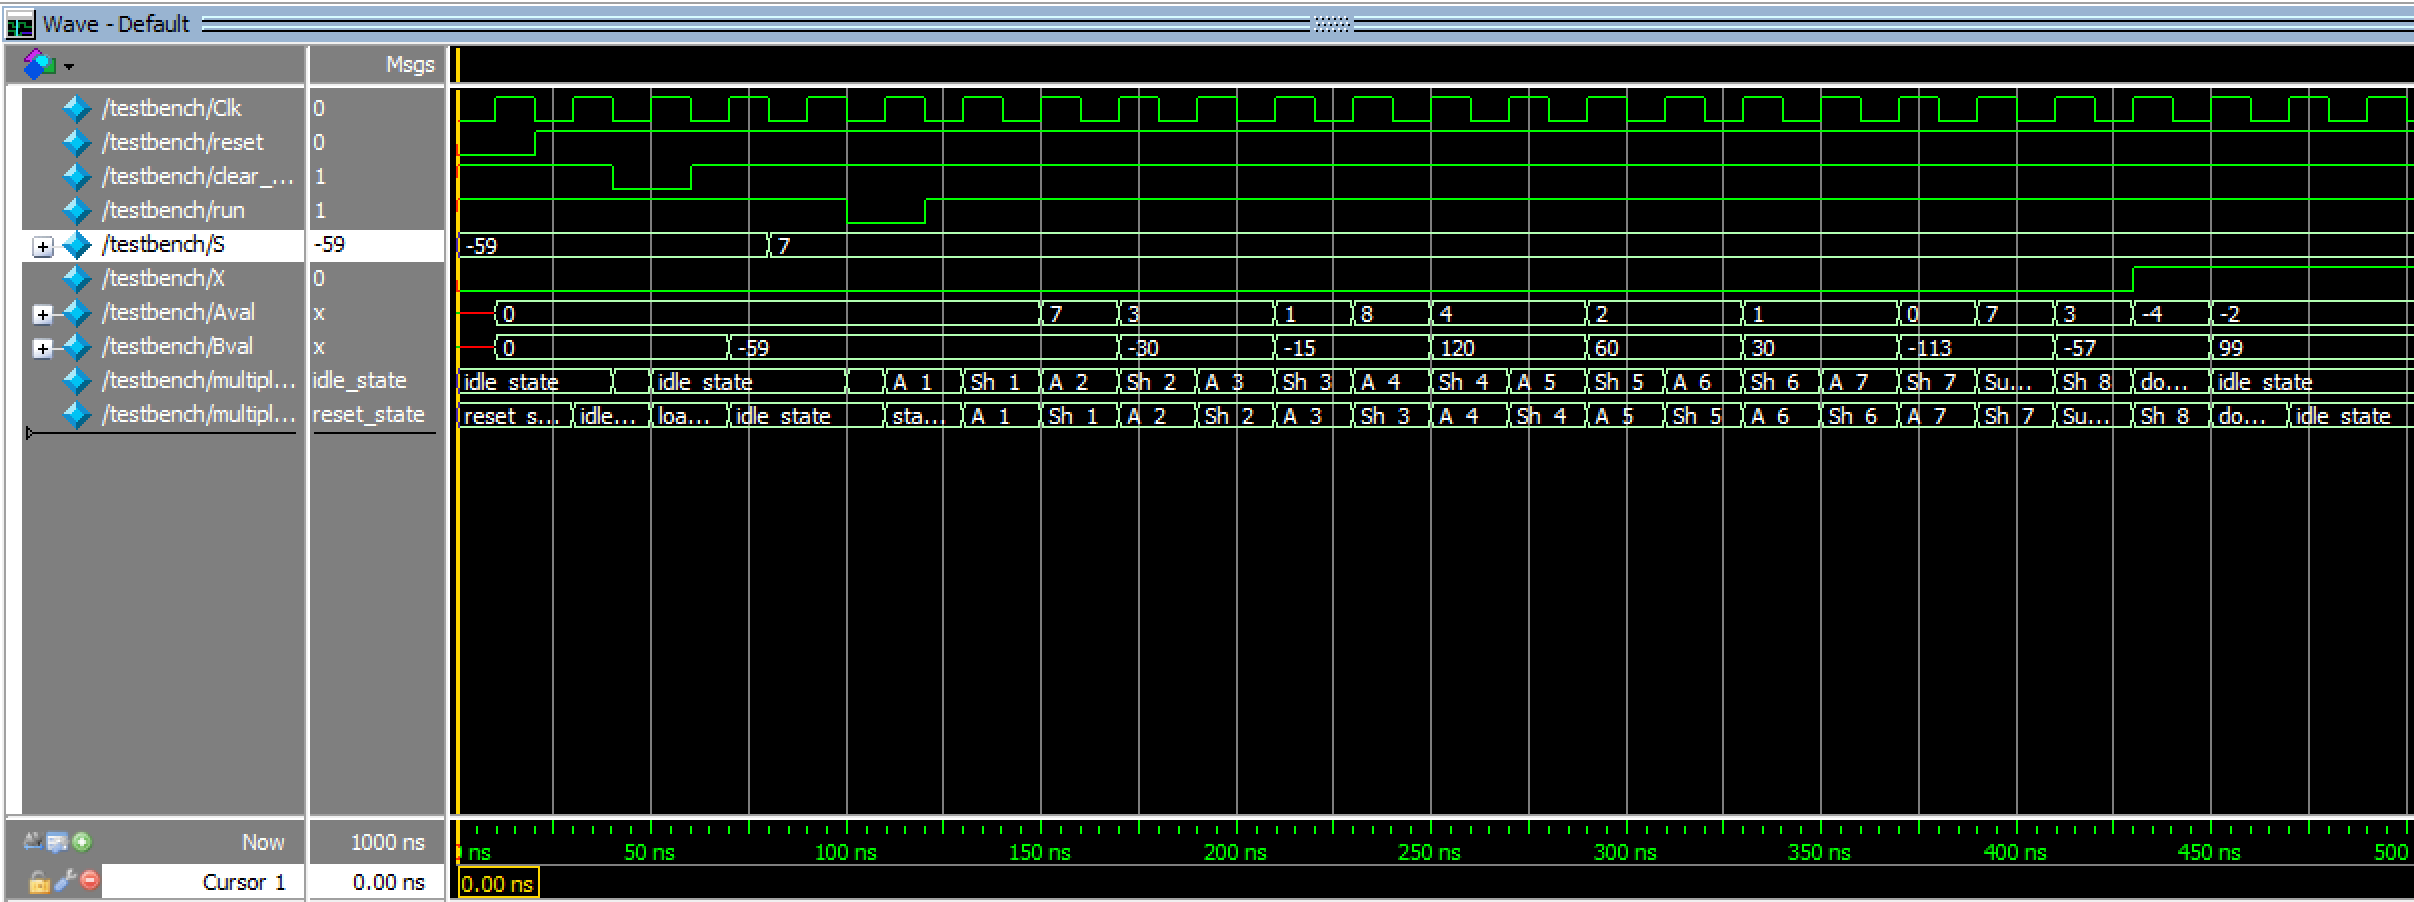
\includegraphics[scale=0.4]{simulation-output.png}
	\caption{ModelSim Simulation Output (+7 * -59)\label{fig:simulation-output}}
\end{figure}
NEED 3 MORE SIMULATIONS!!!!

\begin{figure} [htbp]
	\centering
	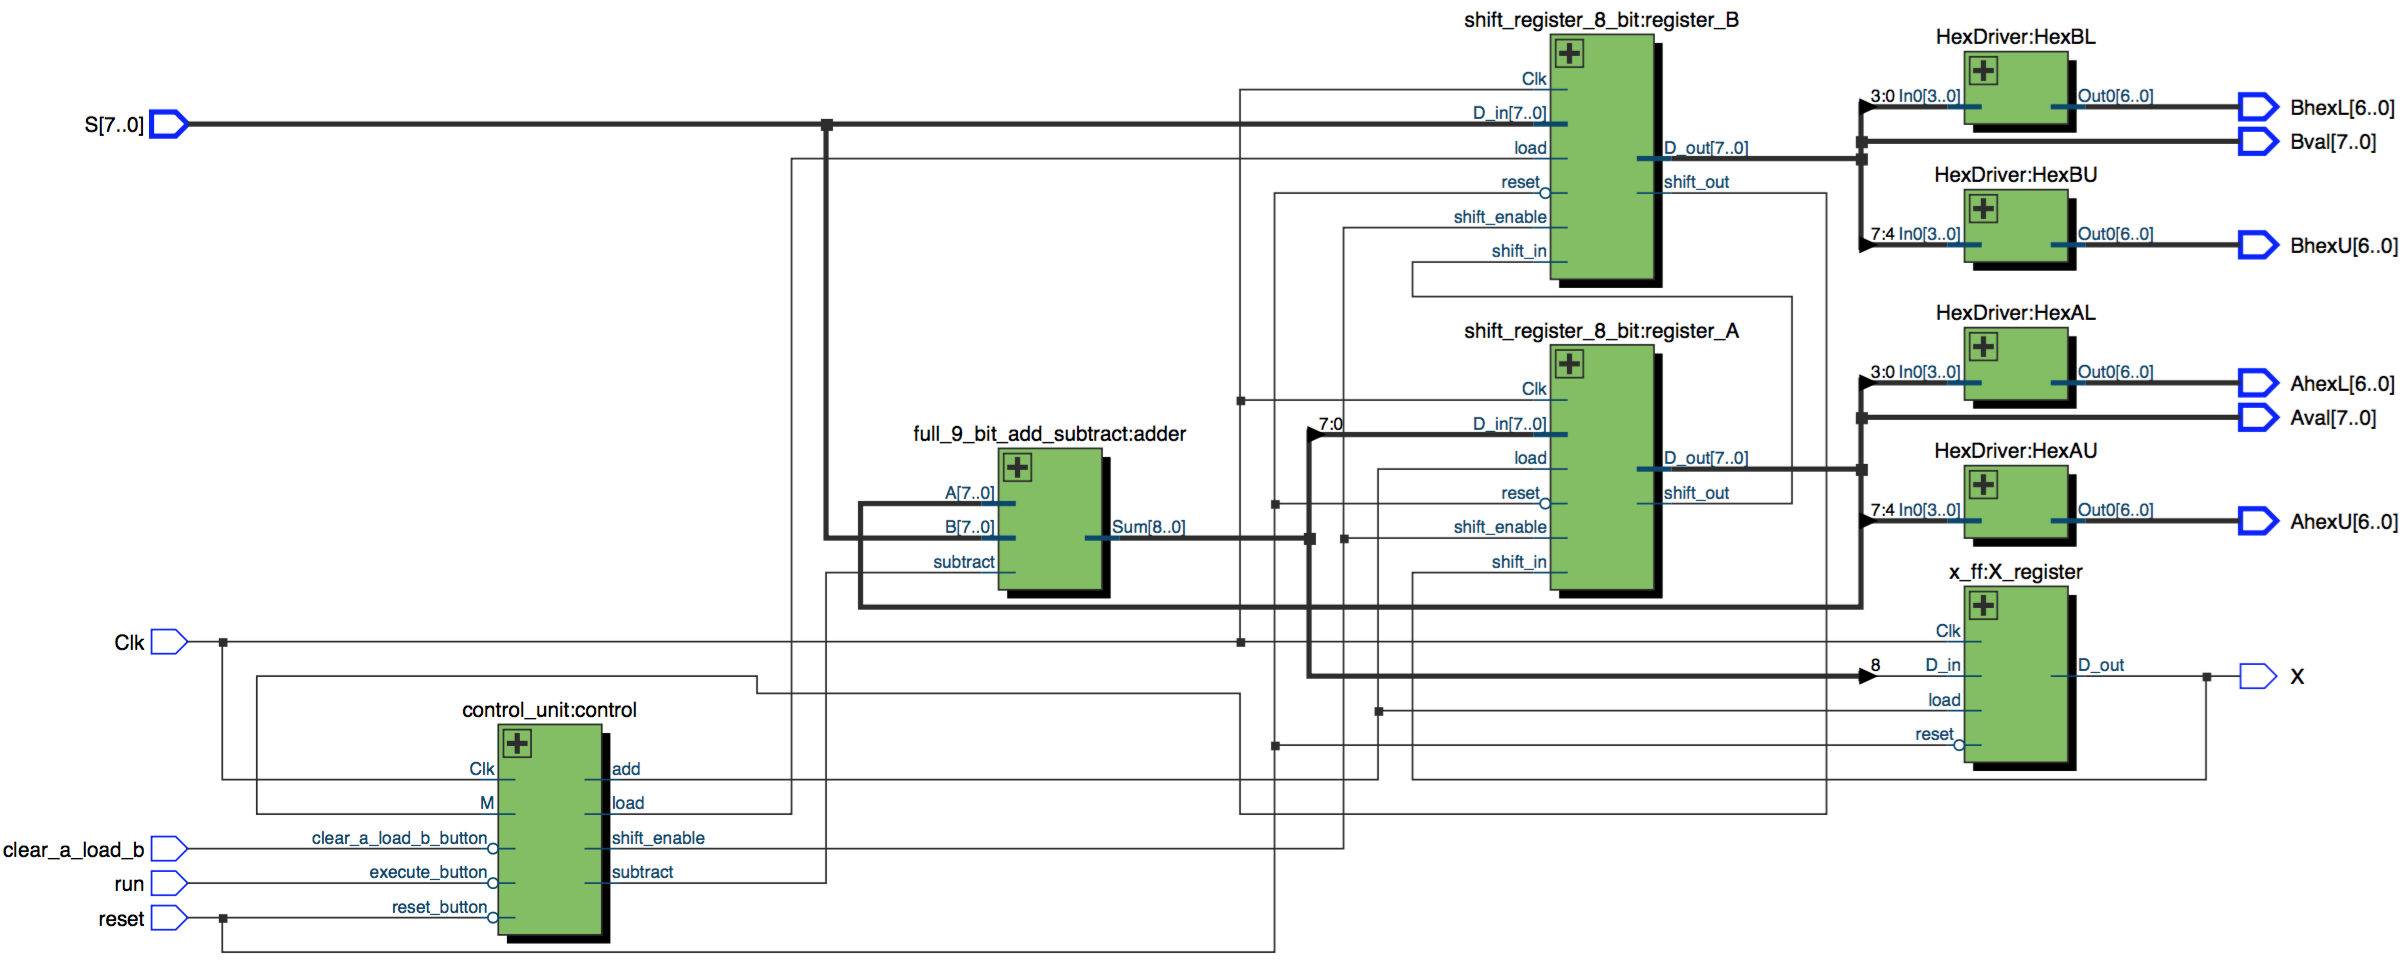
\includegraphics[scale=0.4]{full-multiplier-diagram.png}
	\caption{Full Multiplier Block Diagram\label{fig:full-multiplier-diagram}}
\end{figure}

\begin{figure} [htbp]
	\centering
	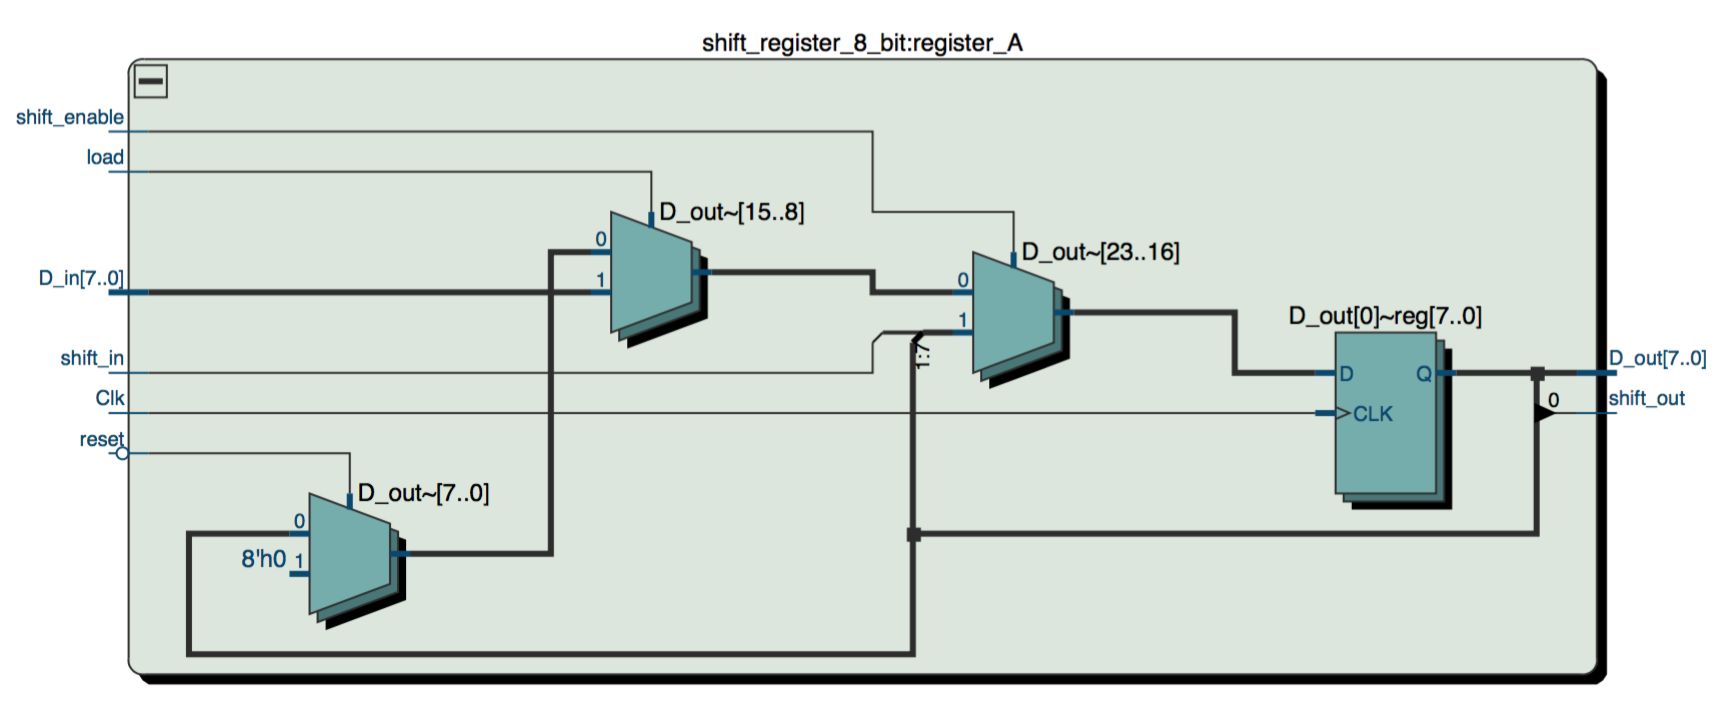
\includegraphics[scale=0.5]{shift-register-diagram.png}
	\caption{Shift Register Block Diagram\label{fig:shift-register-diagram}}
\end{figure}

\begin{figure} [htbp]
	\centering
	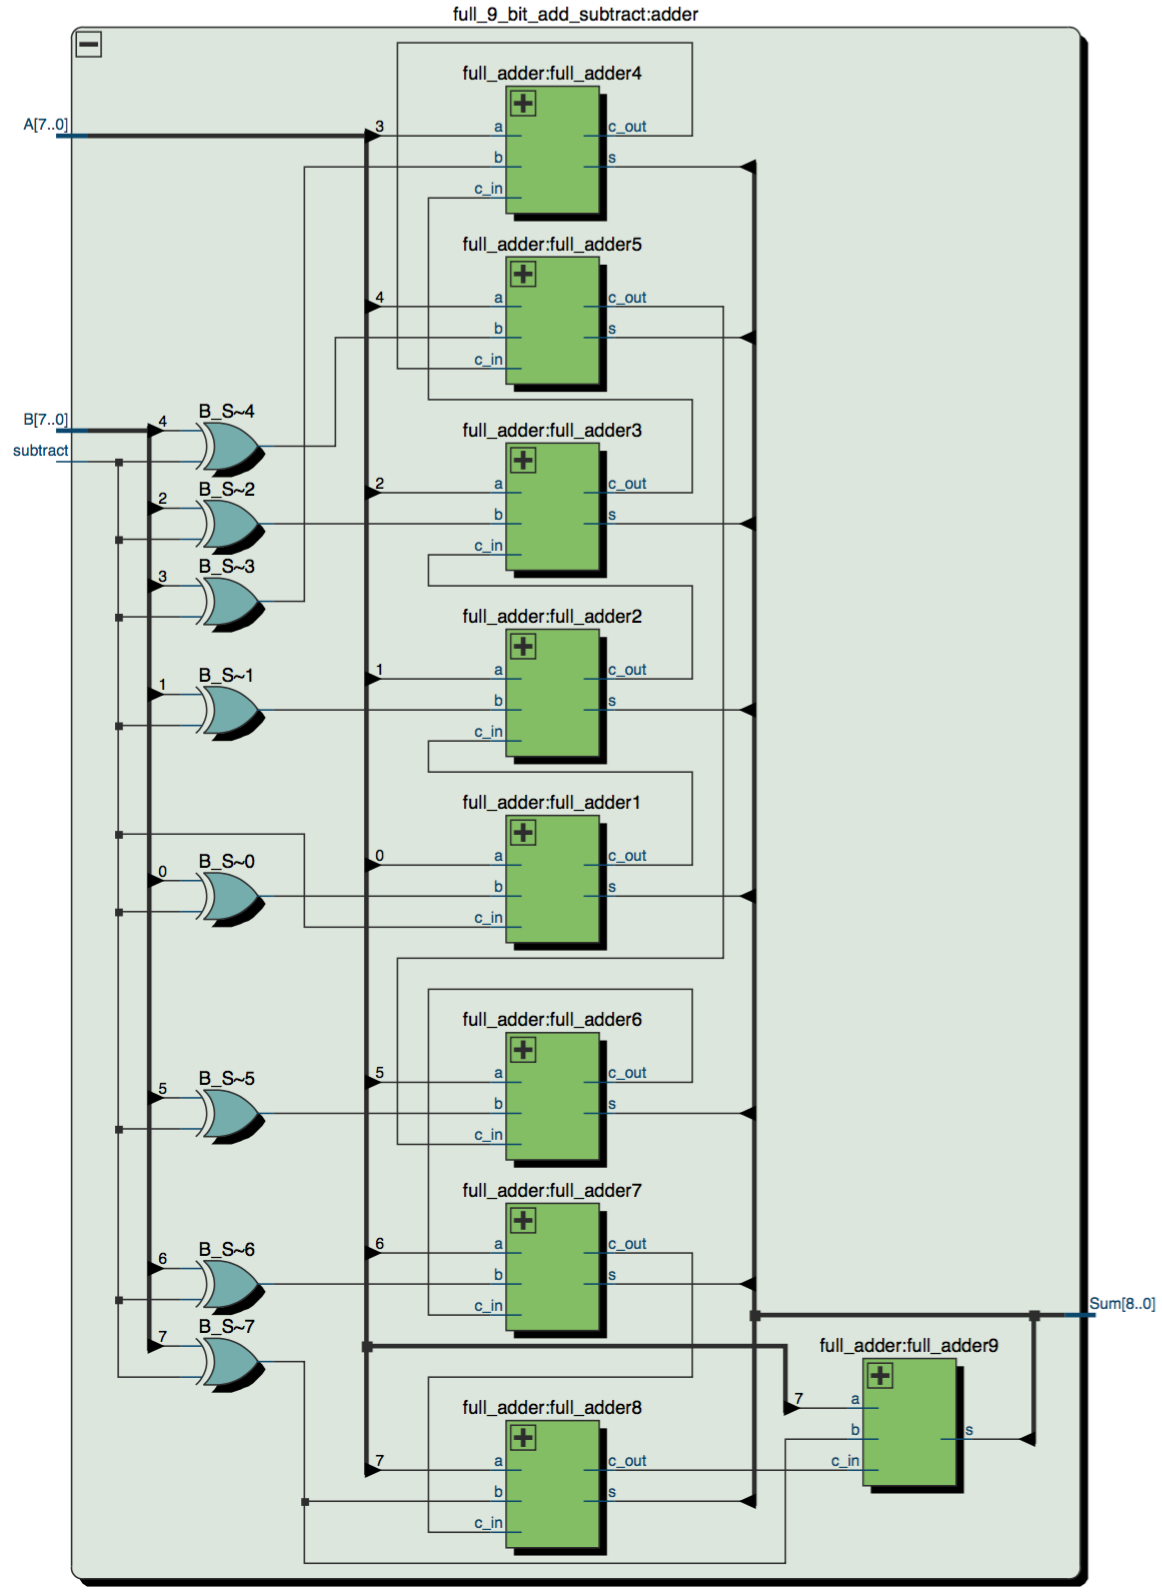
\includegraphics[scale=0.5]{full-adder-subtractor-diagram.png}
	\caption{Full Adder and Subtractor Block Diagram\label{fig:full-adder-subtractor-diagram}}
\end{figure}

\begin{figure} [htbp]
	\centering
	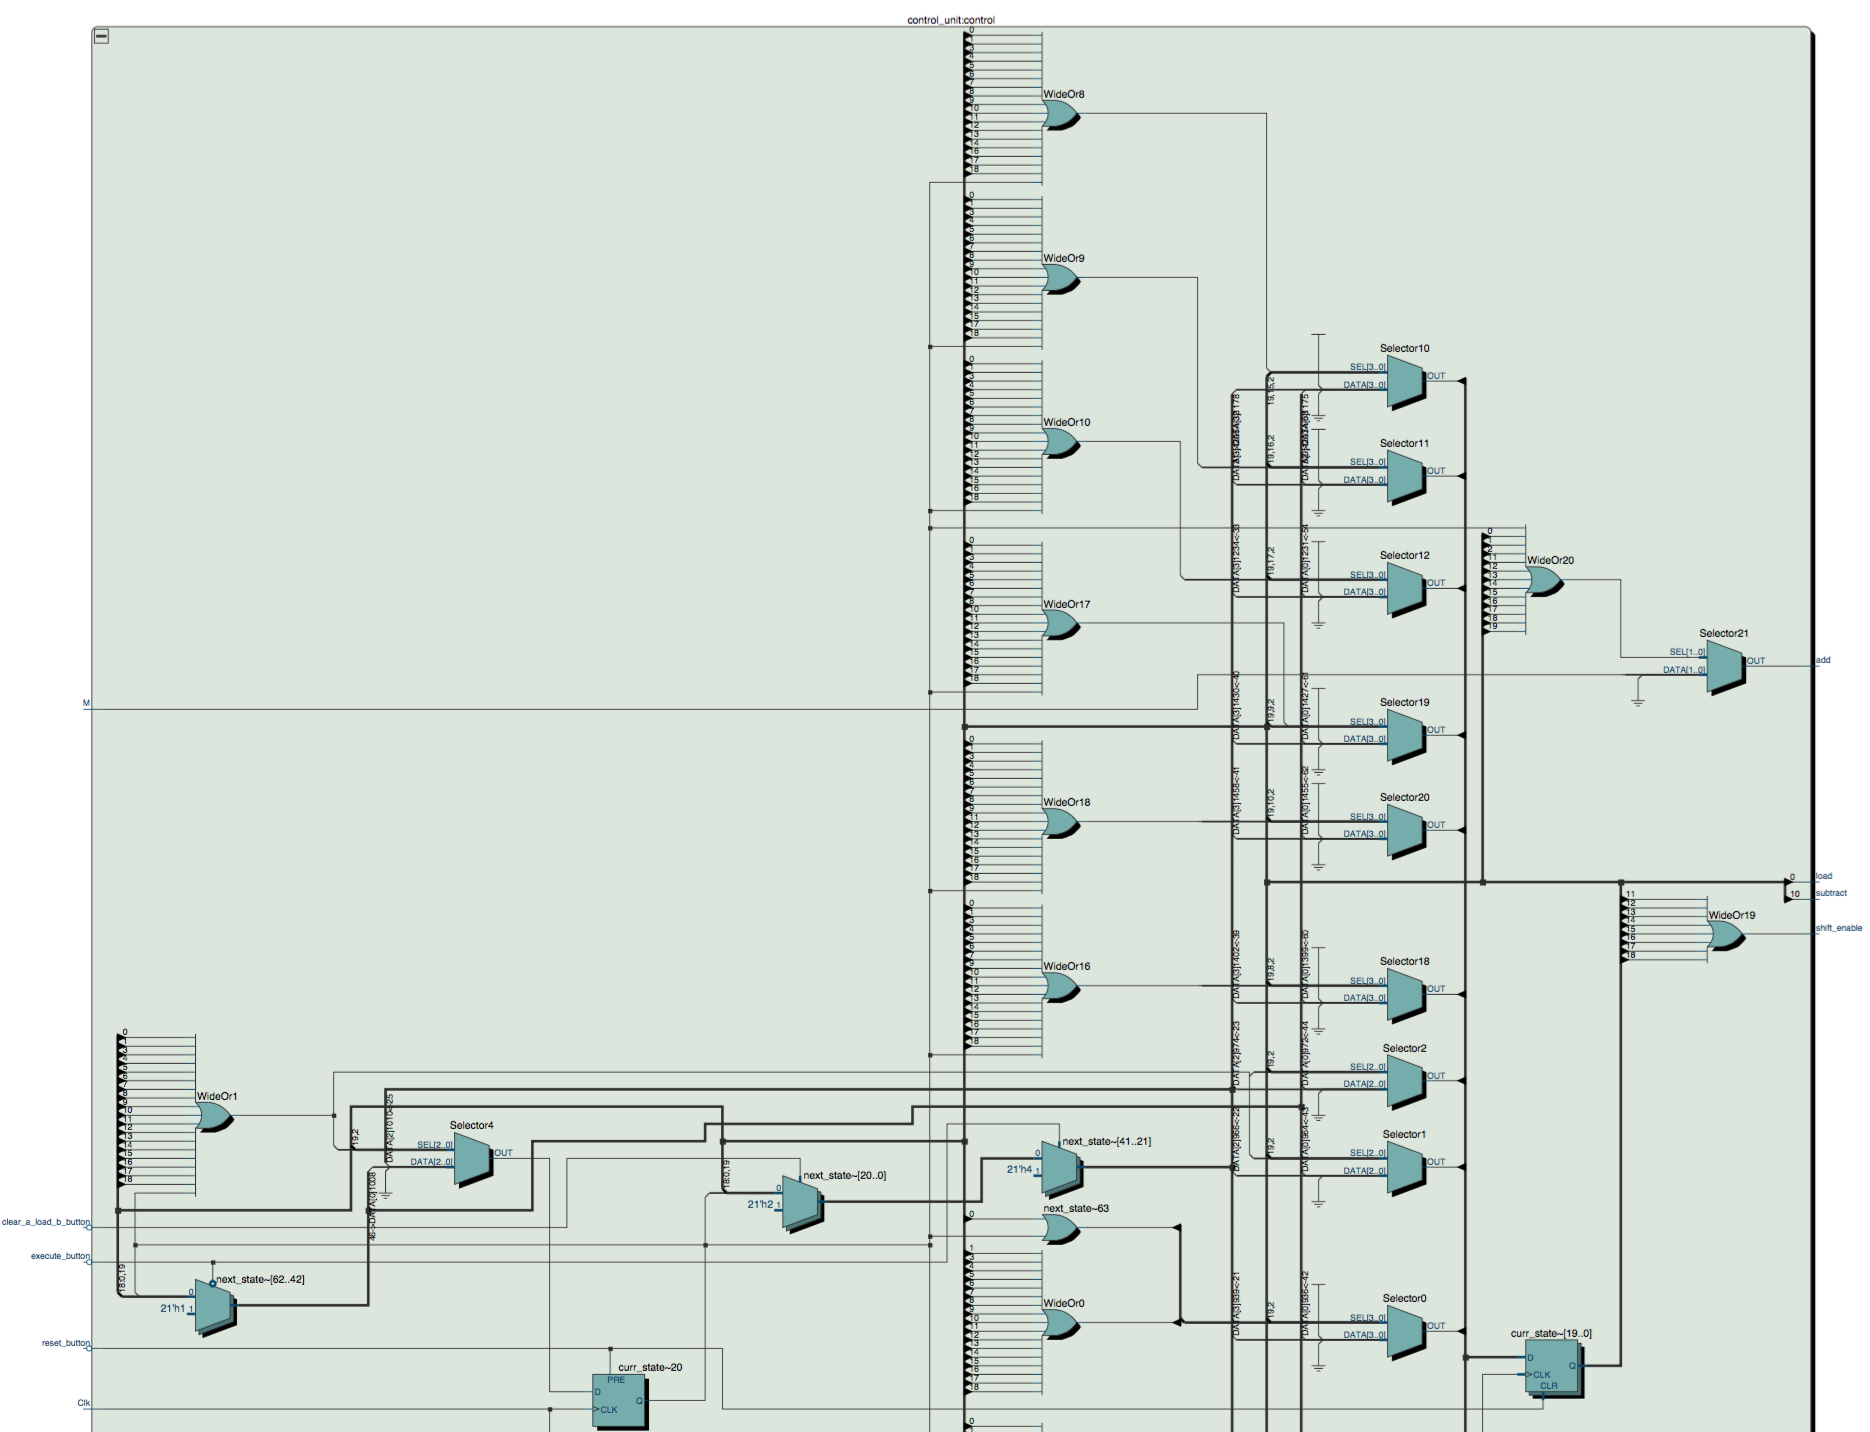
\includegraphics[scale=0.55]{control-unit-top-half-diagram.png}
		\caption{Top Half Control Unit Block Diagram\label{fig:top-half-control}}
\end{figure}

\begin{figure} [htbp]
	\centering
	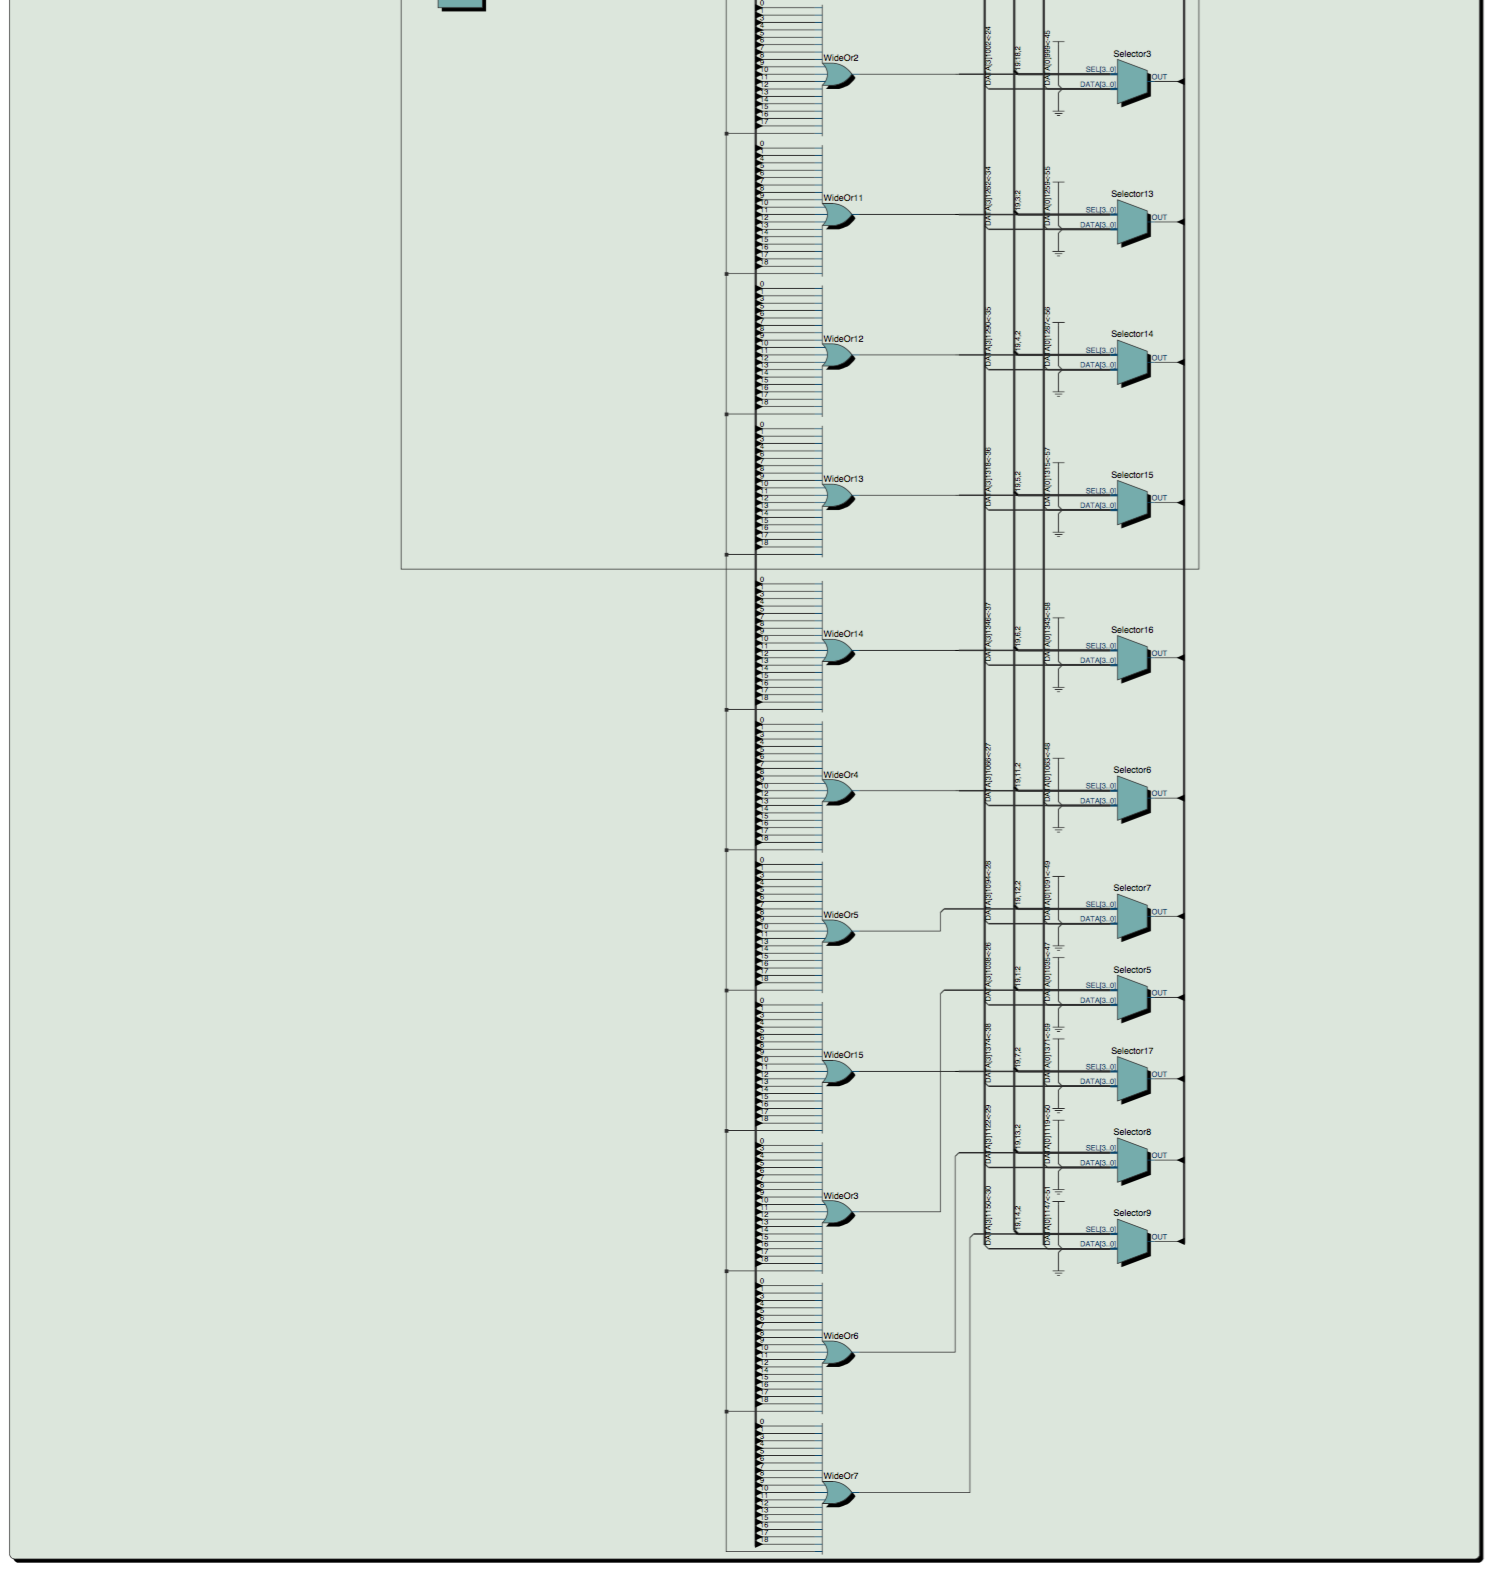
\includegraphics[scale=0.65]{control-unit-bottom-half-diagram.png}
	\caption{Bottom Half Control Unit Block Diagram\label{fig:bottom-half-control}}
\end{figure}

\begin{figure} [htbp]
	\centering
	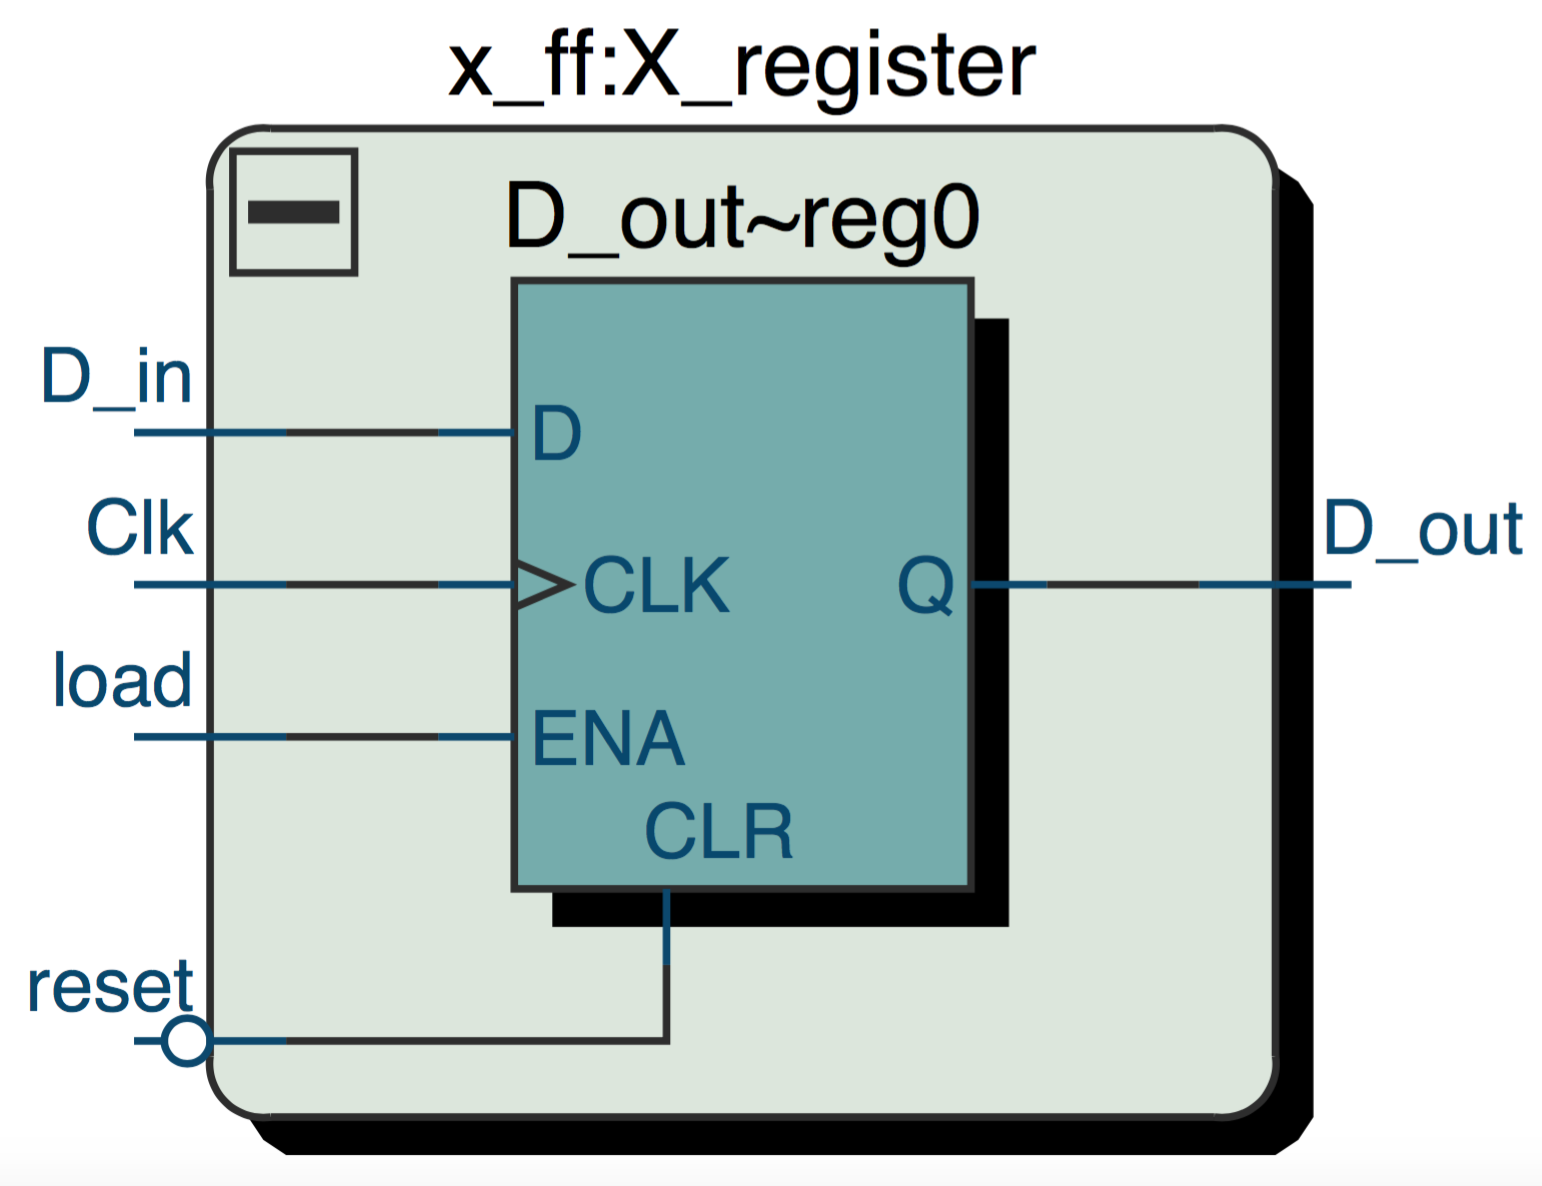
\includegraphics[scale=0.4]{x-ff-diagram.png}
	\caption{X-Bit Flip Flop Block Diagram\label{fig:x-ff-diagram}}
\end{figure}





%SECTION : Bibliography
%Insert Bibliography if needed

\end{document}